\section{Generalizing \sysname{}}
\label{sec:generic}

\revisionshuihai{ We begin by  formalizing the description of the tagging system using notations in
Table~\ref{tab:symbols}. }

Let $A_i$ represent a unique ingress port in the network, {\em i.e.,} switch
$A$'s $i^{th}$ ingress port.  We use a {\em tagged graph} $G(V,E)$ to uniquely
represent a tagging scheme.  Given a tagging scheme, the {\em tagged graph}
$G(V,E)$ is defined as:

\begin{enumerate}
\item $G$ contains a node, $(A_i, x)$, {\em iff.} port $A_i$ may receive packets with tag $x$, and these packets must
be lossless. $V$ is the set of all such nodes.

\item $G$ contains an edge $(A_i, x)\rightarrow(B_j, y)$ {\em iff.} switch $A$ and $B$ are
connected, {\em and} switch $A$ may change a packet's tag from $x$ to $y$ before sending to $B$ (the case $x=y$ also counts).
$E$ is the set of all such edges.

\end{enumerate}

Given a tag $k$, we also define $\{G_k\}$, with vertices $V(G_k)$ and edges
$E(G_k)$:
$$V(G_k) = \{(A_i, k) | \forall A, i\} $$
$$E(G_k) = \{v_0 \rightarrow v_1 | \forall v_0, v_1 \in V(G_k),  v_0 \rightarrow v_1 \in E(G)\} $$
Each tag $k$ is mapped to a unique lossless priority.

Each node has a rule to match on a tag on an ingress port, and assign the packet
to corresponding lossless queue.  In addition, each edge corresponds to a switch
action of setting the tag for the next hop.

\begin{table}[t]
\footnotesize
\centering
\begin{tabular}{|c|c|}
\hline
Symbol & Description \\ \hline
$A_i$ & Switch $A$'s $i^{th}$ ingress port  \\ \hline
$(A_i, x)$ & A node in tagged graph \\ \hline
$(A_i, x)\rightarrow(B_j, y)$ & A tagged edge \\ \hline
$V$ & All tagged nodes  \\ \hline
$E$ & All tagged edges \\ \hline
$G(V, E)$ & Tagged graph \\ \hline
$T$ & Largest tag in $G(V,E)$ \\ \hline
$G_k$ & Partition of $G(V,E)$ for priority $k$ \\ \hline
\end{tabular}
%\vspace{-1em}
\caption{Notations in the formalized description.}
\label{tab:symbols}
	%	\vspace{-3em}
\end{table}



If a packet arrives at $A_i$ with tag $x$, and is destined for port $B_j$, and
there is no corresponding edge in $G(V,E)$, it means that the packet has
traversed on a path that is not in ELP.  Such packets are assigned a special
tag, and all switches assign this tag to lossy priority\footnote{This rule is
always the last one in the TCAM rule list, acting as a safeguard to avoid
unexpected buffer dependency.  See \S\ref{sec:implementation}.}.

In the rest of the section, we will describe how to generate the tagging graph
-- i.e. the tagging rules. But first, we prove that the tagging scheme described
by such a graph is deadlock free, as long as the graph meets two requirements.

\begin{enumerate}

		\item  Any $G_k$ for $G$ {\em must not} have a cycle.  This is
				because each edge in $G_k$ is essentially a buffer dependency --
				whether $A_i$ can dequeue packets depends on whether $B_j$ has
				paused it. A cycle in $G_k$ means cyclic buffer
				dependency.
		\item There must be no link going from
				$G_x$ to $G_y$ if $x>y$.  This means we enforce the order of
				$G_x$ and $G_y$.
\end{enumerate}
These requirements are essentially generalization of the properties
discussed in \S\ref{subsec:specific_deadlock_free}.
\begin{theorem}
Any tag system, defined by $G(V,E)$, that satisfies the above two requirements is deadlock-free.
\end{theorem}

\begin{proof}
\revisionshuihai{ We prove by contradiction. Suppose there exists a tag system,
whose tagged graph $G(V,E)$ satisfies the above two requirements, but is not deadlock-free. This means $G(V,E)$ has a cycle $v_0 \rightarrow v_1 \rightarrow ... \rightarrow v_0$. If traffic traverses all hops in the cycle, the cycle leads into a CBD and can form deadlock. }

%If traffic that covers all hops in the cycle, the cycle leads into a CBD and can form deadlock.

\revisionshuihai{ \textbf{Case 1:}  All the nodes in the cycle have the same tag $t$. According to the first requirement, $G_t$ does {\em not} have a cycle. Contradicted. }

\revisionshuihai{ \textbf{Case 2:} The nodes in the cycle have at least two different tags, $t_0$ and $t_1$. Without loss of generality, we assume $t_0 < t_1$, and $v_i$ has tag $t_0$, $v_j$ has tag $t_1$. Because $v_i$ and $v_j$ belongs to a cycle, there must exist a path going from $v_j$ to $v_i$. Since $t_0 < t_1$, along the path there must exist a hop where the tag decreases. However, according to the second requirement, such a hop cannot exist. Contradicted. }

Case 1 and Case 2 cover all possible scenarios. Thus, we conclude that there does not exist a $G(V,E)$ that satisfies the two requirements but is not deadlock-free.
\end{proof}


%We now describe the algorithm to generate $G(V,E)$ for any given topology, and the ELP set.


\subsection{Generating $G(V,E)$}

\revisionshuihai{ In the next, we describe our algorithm to generate a deadlock-free $G(V,E)$ for any given topology, and the ELP set. }


\begin{figure*}[t]
	\centering
		\subfloat[short for lof][Topology and ELP set.] {
		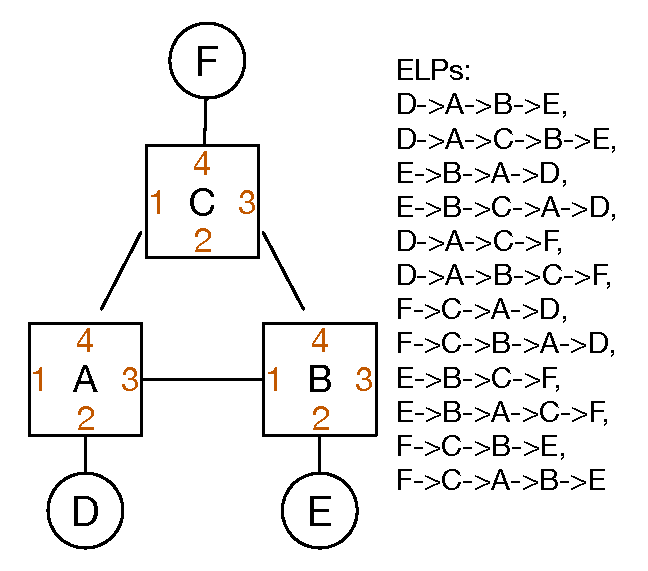
\includegraphics[width=0.26\textwidth] {figs/alo_walkthrough_a}
	}
	\subfloat[short for lof][Output tagged graph by Algorithm~\ref{alg:ttl}.]{
		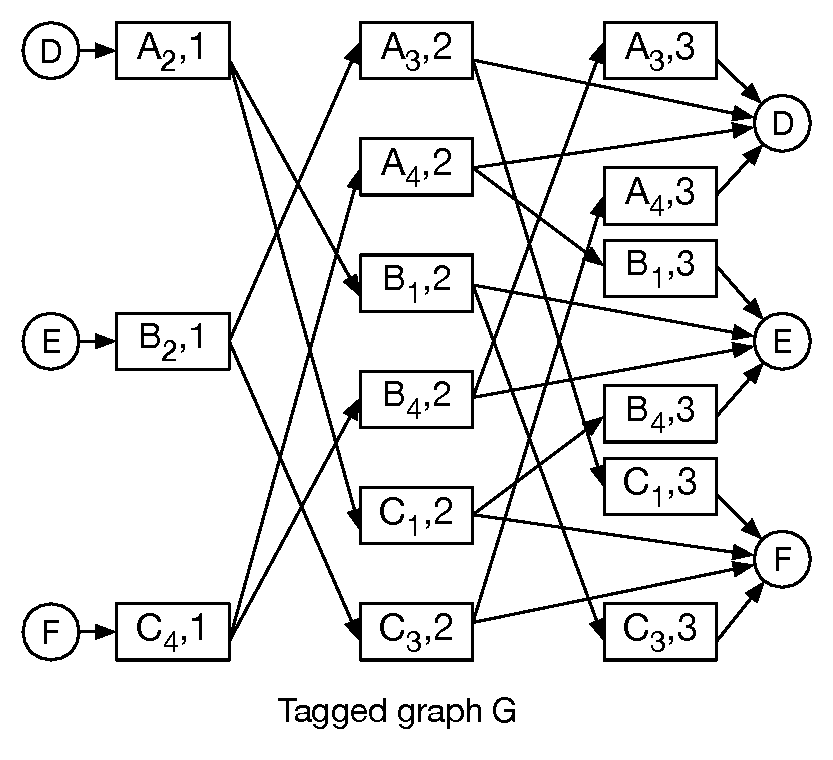
\includegraphics[width=0.28\textwidth] {figs/alo_walkthrough_b}
	}
	\subfloat[short for lof][Output tagged graph by Algorithm~\ref{alg:greedy}.]{
	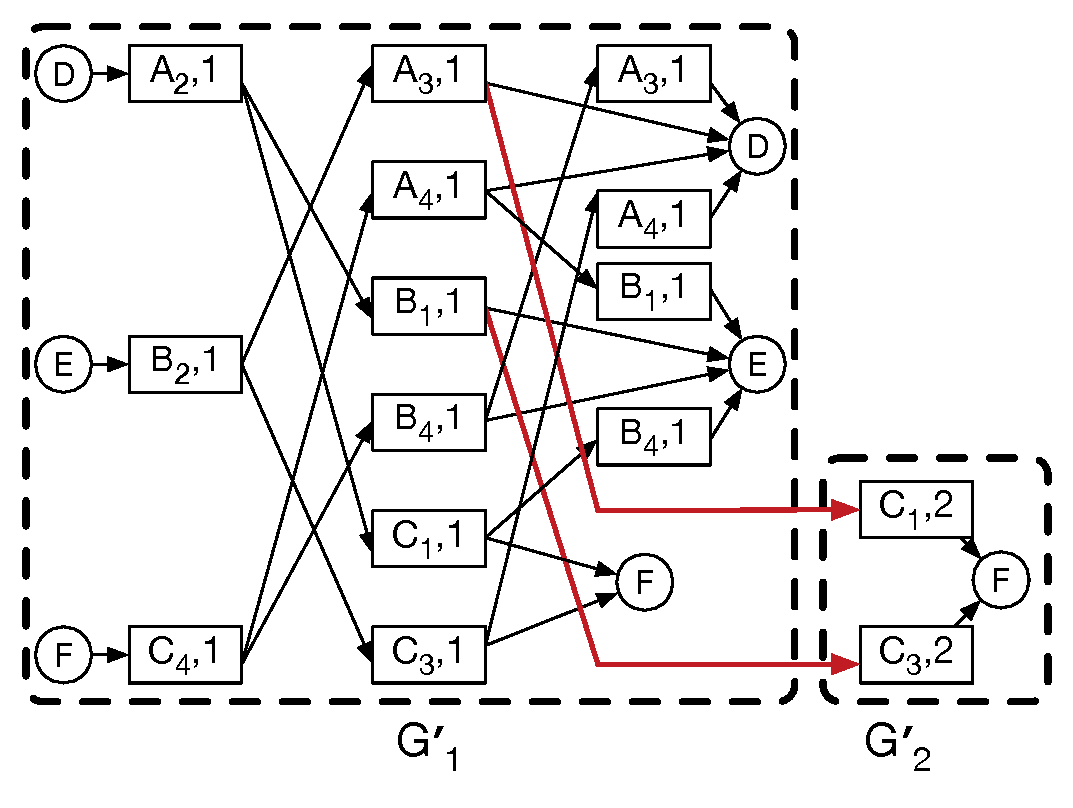
\includegraphics[width=0.34\textwidth] {figs/alo_walkthrough_c}
}
%\vspace{-1em}
	\caption{Walk-through example of the algorithms. Each rectange in (b) and (c) is a (port,tag) pair.}\label{fig:three_node}
%	\vspace{-0.5em}
\end{figure*}



\begin{table*}[t]
\small
\scalebox{0.95}{
    \footnotesize
	\centering
	\begin{tabular}{lll}
		\begin{tabular}{|r|r|r|r|}
			\hline
			Tag&  InPort& OutPort & \textcolor{red}{Newtag} \\
			\hline
			\hline
			1 & 2 & 3 & \textcolor{red}{2} \\
			\hline
			1 & 2 & 4 & \textcolor{red}{2} \\
			\hline
			2 & 3 & 2 & \textcolor{red}{3} \\
			\hline
			2 & 3 & 4 & \textcolor{red}{3} \\
			\hline
			2 & 4 & 2 & \textcolor{red}{3} \\
			\hline
			2 & 4 & 3 & \textcolor{red}{3} \\
			\hline
			3 & 3 & 2& \textcolor{red}{4} \\
			\hline
			3 & 4 & 2 & \textcolor{red}{4} \\
			\hline
			others & others & others & \textcolor{red}{lossy tag} \\
			\hline
			\multicolumn{4}{c}{(a) rules installed in A} \\
		\end{tabular}
		&
		\begin{tabular}{|r|r|r|r|}
			\hline
			Tag&  InPort& OutPort & \textcolor{red}{Newtag} \\
			\hline
			\hline
			1 & 2 & 1 & \textcolor{red}{2} \\
			\hline
			1 & 2 & 4 & \textcolor{red}{2} \\
			\hline
			2 & 1 & 2 & \textcolor{red}{3} \\
			\hline
			2 & 1 & 4 & \textcolor{red}{3} \\
			\hline
			2 & 4 & 1 & \textcolor{red}{3} \\
			\hline
			2 & 4 & 2 & \textcolor{red}{3} \\
			\hline
			3 & 1 & 2& \textcolor{red}{4} \\
			\hline
			3 & 4 & 2 & \textcolor{red}{4} \\
			\hline
			others & others & others & \textcolor{red}{lossy tag} \\
			\hline
			\multicolumn{4}{c}{(b) rules installed in B} \\
		\end{tabular}
		&
		\begin{tabular}{|r|r|r|r|}
			\hline
			Tag&  InPort& OutPort & \textcolor{red}{Newtag} \\
			\hline
			\hline
			1 & 4 & 1 & \textcolor{red}{2} \\
			\hline
			1 & 4 & 3 & \textcolor{red}{2} \\
			\hline
			2 & 1 & 3 & \textcolor{red}{3} \\
			\hline
			2 & 1 & 4 & \textcolor{red}{3} \\
			\hline
			2 & 3 & 1 & \textcolor{red}{3} \\
			\hline
			2 & 3 & 4 & \textcolor{red}{3} \\
			\hline
			3 & 1 & 4 & \textcolor{red}{4} \\
			\hline
			3 & 3 & 4 & \textcolor{red}{4} \\
			\hline
			others & others & others & \textcolor{red}{lossy tag} \\
			\hline
			\multicolumn{4}{c}{(c) rules installed in C} \\
		\end{tabular}
	\end{tabular}
}
%	\vspace{-1em}
	\caption{Tag rewriting rules under Algorithm~\ref{alg:ttl}. Tag ``4'' will only appear on destination servers.}
	\vspace{-2em}
	\label{table:tagging_table}
\end{table*}

For general graph without structure information, a straightforward tagging
system~\cite{karol2003prevention} is to monotonically increase the tag (thus,
the priority) at every hop, as described in Algorithm~\ref{alg:ttl}.

\begin{algorithm}[t]
	\small
    \KwIn{Topology and $ELP$}
	\KwOut{A tagged graph $G(V, E)$}
	$V \gets Set()$\;
	$E \gets Set()$\;
	\For{each path $r$ in $ELP$} {
		$tag \gets 1$\;
		\For{each hop $h$ in $r$} {
			$V \gets V \cup \{(h, tag)\}$\;
			$E \gets E \cup \{lastHop\rightarrow(h, tag)\}$\;
			$tag \gets tag+1$\;
		}
	}
	\Return{$G(V, E)$}\;
    \caption{A brute-force tagging system that decreases the tag by one on every hop.}
	\label{alg:ttl}
\end{algorithm}




It is easy to verify that the graph generated by this algorithm meets the two
requirements specified earlier, and thus it guarantees deadlock freedom.
Figure~\ref{fig:three_node} shows a small example, including the topology, the
ELP set, the generated graph, and the corresponding rule
lists for each node.

Of course, with just this basic algorithm, we may end up with too many tags
(i.e. lossless priorities) -- in fact, as many as the longest path length in
lossless routes. This is why we need three lossless priorities for
the simple example in Figure~\ref{fig:three_node}(b). In a three-layer Clos
network, the longest up-down path has 5 hops, so Algorithm~\ref{alg:ttl} will use 5
priorities just to support up-down routing. We now show how to combine tags to
reduce the number of lossless queues needed.

\subsection{Reducing the number of lossless queues}
%%comment: i do not see the use of micropath before. hence i am recoving it here.
%%comment: need to discuss and decide the smallest tag. I believe it should start from 1. 0 is reserved for lossy.
%%comment: change subspace  to subgraph? it is a dag, hence a graph. but it is not a space.




Algorithm~\ref{alg:greedy} uses a greedy heuristic to combine the tags generated
by Algorithm~\ref{alg:ttl} to reduce the number of lossless queues required.  It
greedily combines as many nodes in $G(V,E)$ as possible into each path segment
under CBD-free constraint. To ensure the monotonic property, we start
from combining the nodes with smallest tag, 1 and proceed linearly to consider
all tags up to $T$, which is the largest tag number used in $G(V,E)$.

\begin{algorithm}[t]
	\small
    \KwIn{The brute-force tagged graph $G(V, E)$ with largest tag $T$}
	\KwOut{A new tagged graph $G'(V', E')$ that has small $|\{G'_k\}|$}
	Initialize $V'$, $E'$, $V_{tmp}$, $E_{tmp}$ as empty $Set()$\;
	$t' \gets 1$\;
	\For{$t \gets 1$ \textbf{to} $T$} {
		\For{each $(A_i, t)$ in $V$ whose tag is $t$} {
			$V_{tmp} \gets V_{tmp} \cup \{(A_i, t')\}$\;
			$E_{tmp} \gets E_{tmp} \cup \{$edges of $(A_i, t)$, change $t$ to $t'\}$\;
			\uIf{$G_{tmp}(V_{tmp}, E_{tmp})$ is acyclic} {
				$V' \gets V' \cup \{(A_i, t')\}$\;
				$E' \gets E' \cup \{$edges of $(A_i, t)$, change $t$ to $t'\}$\;
			}
			\Else{
				$V' \gets V' \cup \{(A_i, t'+1)\}$\;
				$E' \gets E' \cup \{$edges of $(A_i, t)$, change $t$ to $t'+1\}$\;
				$V_{tmp} \gets V_{tmp} \backslash \{(A_i, t')\}$\;
				$E_{tmp} \gets E_{tmp} \backslash \{$edges of $(A_i, t')\}$\;
			}
		}
		\uIf{$V'$ contains nodes of tag $t'+1$} {
			$V_{tmp} \gets \{$nodes in $V'$ with tag $t'+1\}$\;
			$E_{tmp} \gets \{$edges in $V'$, both ends have tag $t'+1\}$\;
			$t' \gets t'+1$\;
		}
	}
	\Return{$G'(V', E')$}\;
    \caption{Greedily minimizing the number of tags by merging brute-force tags.}
	\label{alg:greedy}
\end{algorithm}

%\begin{figure}[t]
%	\centering
%	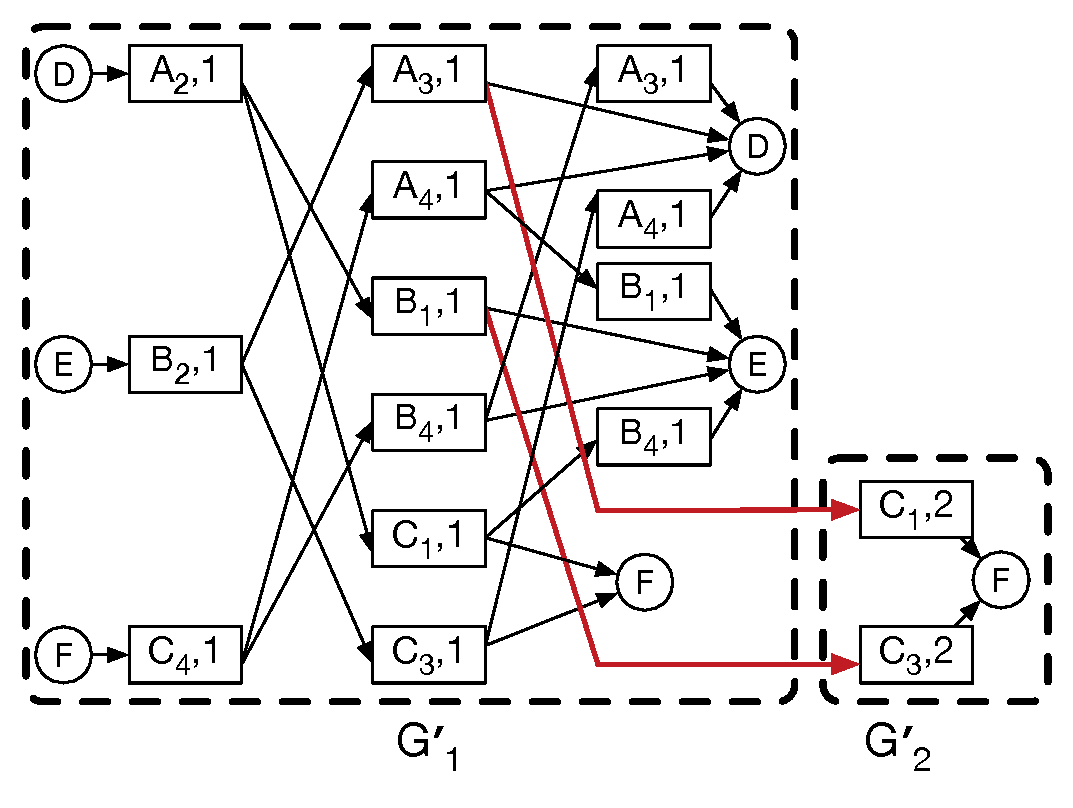
\includegraphics[width=0.48\textwidth] {figs/alo_walkthrough_c}
%	\caption{Algorithm~\ref{alg:greedy} output for the example in Figure~\ref{fig:three_node}.}
%	\label{fig:greedy}
%	\vspace{-1em}
%\end{figure}

\begin{table*}[t]
\small
\scalebox{0.95}{
	\footnotesize
	\centering
	\begin{tabular}{lll}
		\begin{tabular}{|r|r|r|r|}
			\hline
			Tag&  InPort& OutPort & \textcolor{red}{Newtag} \\
			\hline
			\hline
			1 & 2 & 3 & \textcolor{red}{1} \\
			\hline
			1 & 2 & 4 & \textcolor{red}{1} \\
			\hline
			1 & 3 & 2 & \textcolor{red}{1} \\
			\hline
			1 & 3 & 4 & \textcolor{red}{2} \\
			\hline
			1 & 4 & 2 & \textcolor{red}{1} \\
			\hline
			1 & 4 & 3 & \textcolor{red}{1} \\
			\hline
			others & others & others & \textcolor{red}{lossy tag} \\
			\hline
			\multicolumn{4}{c}{(a) Rules installed in A} \\
		\end{tabular}
		&
		\begin{tabular}{|r|r|r|r|}
			\hline
			Tag&  InPort& OutPort & \textcolor{red}{Newtag} \\
			\hline
			\hline
			1 & 2 & 1 & \textcolor{red}{1} \\
			\hline
			1 & 2 & 4 & \textcolor{red}{1} \\
			\hline
			1 & 1 & 2 & \textcolor{red}{1} \\
			\hline
			1 & 1 & 4 & \textcolor{red}{2} \\
			\hline
			1 & 4 & 1 & \textcolor{red}{1} \\
			\hline
			1 & 4 & 2 & \textcolor{red}{1} \\
			\hline
			others & others & others & \textcolor{red}{lossy tag} \\
			\hline
			\multicolumn{4}{c}{(b) Rules installed in B} \\
		\end{tabular}
		&
		
		\begin{tabular}{|r|r|r|r|}
			\hline
			Tag&  InPort& OutPort & \textcolor{red}{Newtag} \\
			\hline
			\hline
			1 & 4 & 1 & \textcolor{red}{1} \\
			\hline
			1 & 4 & 3 & \textcolor{red}{1} \\
			\hline
			1 & 1 & 3 & \textcolor{red}{1} \\
			\hline
			1 & 1 & 4 & \textcolor{red}{1} \\
			\hline
			1 & 3 & 1 & \textcolor{red}{1} \\
			\hline
			1 & 3 & 4 & \textcolor{red}{1} \\
			\hline
			2 & 1 & 4 & \textcolor{red}{2} \\
			\hline
			2 & 3 & 4 & \textcolor{red}{2} \\
			\hline
			others & others & others & \textcolor{red}{lossy tag} \\
			\hline
			\multicolumn{4}{c}{(c) Rules installed in C} \\
		\end{tabular}
		
	\end{tabular}
%	\vspace{-1em}
}
	\caption{Tag rewriting rules generated by Algorithm~\ref{alg:greedy} (without compression).}
	\vspace{-2em}
	\label{table:tagging_table2}
\end{table*}

The new tag $t'$ also starts from 1. In every iteration, we check all nodes with
the same tag value $t$. $V_{tmp}$ and $E_{tmp}$ is the ``sandbox''. For every
node, we add it to $V_{tmp}$ and $E_{tmp}$ and check whether adding it to
$G'_{t'}$ will lead to a cycle within $G'_{t'}$. If not, we re-tag the node to
be $t'$. Otherwise, we re-tag the node to be $t'+1$.  Re-tagging the node to be
$t'+1$ does not cause a cycle in $G'_{t'+1}$, because all nodes in $G'_{t'+1}$
so far have the same old tag of $t$, which means there is no edge between them.
At the end of each iteration, if there are nodes being re-tagged as $t'+1$, we
move on to add nodes into $G'_{t'+1}$ in the next iteration.  This ensures that
the monotonic property will still hold after combination.

In Figure~\ref{fig:three_node}(c) we see Algorithm~\ref{alg:greedy} in action to
minimize the $G(V,E)$ from Figure~\ref{fig:three_node}. We see that the number
of tags is reduced to {\em two}.

\subsection {Analysis}
\label{subsec:caveats}




\para{Algorithm runtime:} Algorithm~\ref{alg:greedy} is efficient. Recall that
$T$ is the largest value of tag in $G(V,E)$. Let $S$, $L$ and $P$ be the number 
of switches, the number of links and the number of ports a switch has in the
original topology, respectively. Then, $G(V,E)$ can have at most $L \times T$
nodes.  Each node will be examined exactly once for checking whether $G_{tmp}$
is acyclic.  Checking whether $G_{tmp}$ is acyclic with a newly added node
requires a Breadth-First Search, with runtime complexity of $O(|V_{tmp}| +
|E_{tmp}|)$. $|V_{tmp}|$ is bounded by the number of links $L$, and $|E_{tmp}|$ 
is bounded by the number of pairs of incident links $L \times P$, in the network. Thus,
the total runtime complexity is $O(L \times T \times (L+L \times P))$. Note that $T$
itself is bounded by the length of the longest path in $ELP$.


%\para{Algorithm runtime:}. Algorithm~\ref{alg:greedy} is efficient. Recall that
%$mT$ is the largest value of tag in $G(V,E)$. Let the number of links in the
%original topology be $L$. Then, $G(V,E)$ can have at most have $L \times mT$
%nodes.  Each node will be examined exactly once for checking whether $G_{tmp}$
%is acyclic.  Checking whether $G_{tmp}$ is acyclic with a newly added node
%requires a Breadth-First Search, with runtime complexity of $O(|V_{tmp}| +
%|E_{tmp}|)$. $|V_{tmp}|$ is bounded by the number of switches $S$, and
%$|E_{tmp}|$ is bounded by the number of links, $L$, in the network.  Therefore,
%the total runtime complexity is $O(L \times mT \times (S+L))$. Note that $mT$
%itself is bounded by the length of the longest path in $ELP$.


\revisionshuihai{ \para{Number of tags:} Algorithm~\ref{alg:greedy} is not optimal, but works well in practice. For example, it gives optimal results for BCube topology without requiring any BCube-specific changes -- a $k$-level BCube with default routing only needs $k$ tags to prevent deadlock. The results are promising even for unstructured topology like Jellyfish. Using Algorithm~\ref{alg:greedy}, a 2000-node Jellyfish topology with shortest-path routing requires only 3 tags to be deadlock-free (\S\ref{sec:eval}). }


%\para{Number of tags:} Algorithm~\ref{alg:greedy}, while not optimal, works well in practice. For example, it gives optimal results for BCube topology without requiring any BCube-specific changes -- a $k$-level BCube needs $k$ tags to prevent deadlock with default routing. The results are promising even for unstructured topology like Jellyfish. Jellyfish with 2000 nodes require only 3 tags with shortest-path routing (\S\ref{sec:eval}).



\para{Number of rules:} From the conceptual switch model, a switch needs InPort 
(ingress port number), OutPort (egress port number), and the current Tag to decide the next Tag.
Hence it seems the number of rules needed per switch is $n(n-1)\times
\frac{m(m-1)}{2}$, where $n$ is the number of switch ports and $m=|G'_{k}|$ is
the number of Tags. We will show in \S~\ref{sec:implementation} that the number
of rules can be compressed to  $n\times \frac{m(m-1)}{2}$, by taking advantage
of the bit masking technique supported in commodity ASICs.
Table~\ref{table:tagging_table2} shows the rules before compression.

\revisionshuihai{  \para{Optimality:} Algorithm~\ref{alg:greedy} may not return the optimal solution.  Consider the example shown in Figure~\ref{fig:nonoptimal}.  If ELP set consists of shortest and ``1-bounce'' paths, we know the optimal tagging system
only requires {\em two} lossless queues. However, the greedy algorithm will
output a tagging system that requires {\em three} lossless queues. The reason is that
Algorithm~\ref{alg:greedy} does not combine bounces that happen when the packet
is going up and when the packet is coming down. }

\revisionshuihai{ For example, as shown in Figure~\ref{fig:nonoptimal}, the bounce of green flow
will force Algorithm~\ref{alg:greedy} to create a new tag for the first two hops,
since the third hop, which is a bouncing hop, may lead to CBD.  However, the
blue flow bounces at the last two hops and will force Algorithm~\ref{alg:greedy} to create another new tag. Thus, Algorithm~\ref{alg:greedy} generates three tags, requiring three lossless queues. }

The fundamental reason for this is that generic algorithm does not fully utilize
the inherent characteristics of structured topology like Clos. We have not been
able to find an optimal solution to this problem (nor have we been able to prove
that the problem is NP-hard) -- although we can create topology-specific
solutions, as seen in \S\ref{sec:specific}. 

%and Appendix~\ref{sec:clos_optimal}

\revisionshuihai{However, we do note that the number of tags in the solution generated by
Algorithm~\ref{alg:greedy} is an upper bound on the optimal solution. } Without
any assumptions, the worst case is the same as using the brute-force solution,
which requires as many tags as the length of longest lossless route, $T$.
However, if we know that the smallest cycle in lossless routes is longer than
$l$, the output number of tags is bounded by $\lceil T/l \rceil$. We omit the
proof.

\begin{figure}[t]
	%\vspace{-0.1in}
	\centering
	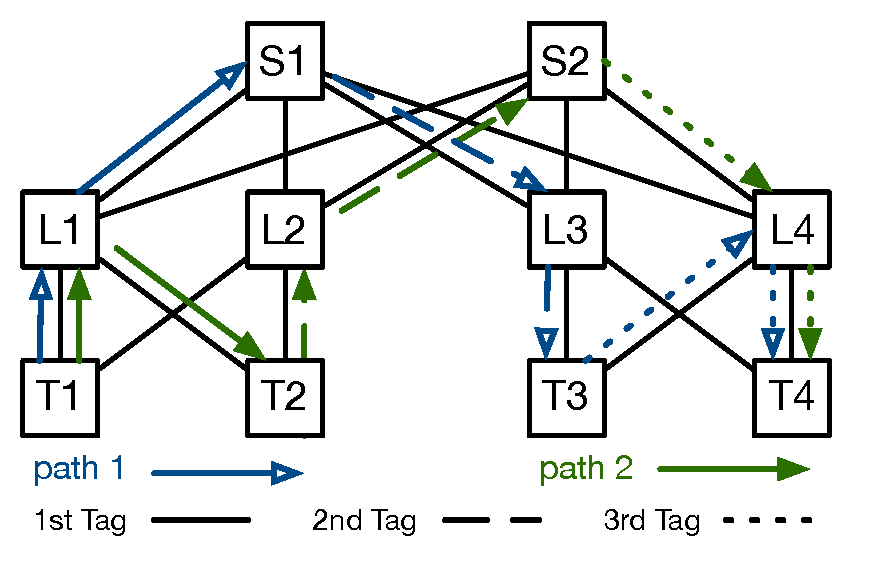
\includegraphics[width=0.45\textwidth] {figs/nonoptimal_example}
	%	\vspace{-0.15in}
	\caption{Algorithm~\ref{alg:greedy} does not output optimal result for Clos with 1-bounce paths.}
	\label{fig:nonoptimal}
	%	\vspace{-0.2in}
\end{figure}